\documentclass[letterpaper,14pt]{memoir}
\usepackage[margin=0.75in]{geometry}
\usepackage{hyperref}
\usepackage{graphicx}
\usepackage{fancyvrb}
\urlstyle{same} % keeps link style same as rest of document
\counterwithout{subsection}{chapter}

\begin{document}

% \begin{flushright}
% \small{ \today }
% \end{flushright}

\begin{center}
\huge{SAVI Manual}\\[0.1in]
\small{Oliver (oe2118@cumc.columbia.edu)\\August 2015}
% \normalsize{ \today }
\end{center}
   
\subsection{Introduction}

SAVI, \emph{statistical algorithm for variant identification}, is a program for calling variants in genomic sequencing data. Why run SAVI? In a word, SAVI is for finding needles in haystacks. It can boil a very large dataset into a small list of mutations. In bioinformatics, \emph{calling variants} can mean two different things: (1) simply enumerating all differences between some sequence data and a reference; and (2) determining which of those differences are significant and not likely to be error. SAVI does the later, while a program like \texttt{samtools mpileup} will do the former. In practice, SAVI is a way of sifting through large amounts of data to pull out the significant mutations using a Bayesian probability model. A common use case is identifying deleterious mutations in cancer, given normal and tumor sequence data---an often-encountered problem in bioinformatics. The output of SAVI is a list of candidate genomic alterations each annotated with a probability of how likely it is to be real.

SAVI works with standard bioinformatic file formats. As input, the SAVI pipeline takes bam files and it produces vcf, as well as tsv, files as output. In the output vcf files, the SAVI probabilities are added in the INFO field.

If you're interested in the mathematical underpinings of SAVI, you can read about it in \href{https://www.biomedcentral.com/1752-0509/7/S2/S2}{this BMC Systems Biology paper} \cite{saviref}.

\subsection{General Variant Calling Pipelines in Bioinformatics}\label{General Variant Calling}

Let's look at a schematic for a general variant calling pipeline in bioinformatics, paying attention to the input/output file formats as data moves through it:

\begin{flushright}
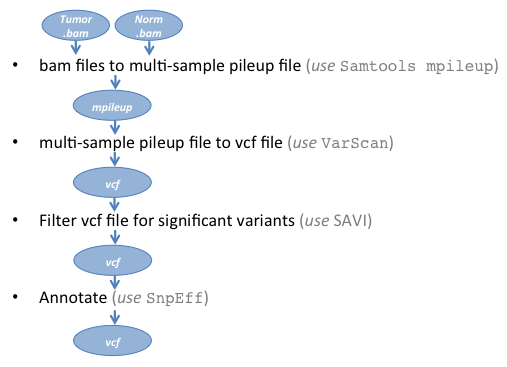
\includegraphics[scale=0.75]{pipeline_507.png}
\end{flushright}

\noindent To flesh this out, a typical workflow might be:

\begin{itemize}
\tightlist
\item
  align reads to reference with bwa or bowtie to produce bam files
\item
  produce a (multi-sample) pileup file with \texttt{samtools mpileup}
\item
  change the pileup file into vcf format with bcftools or VarScan
\item
  filter the vcf for significant variants
\item
  annotate the filtered vcf file with SnpEff.
\end{itemize}

\noindent How the filtering is done is the crux of this problem and determines whether or not this pipeline will be lousy or good.
  
\subsection{The SAVI Pipeline}\label{The SAVI Pipeline}

The SAVI pipeline is organized into 5 main steps and loosely follows the schema of the general variant calling pipeline described in the previous section. Confusingly, we use \textit{``SAVI"} to mean two things: (1) as a shorthand for the pipeline as a whole; and (2) more precisely, to refer to the all-important step 4 of this multi-step pipeline---the one that filters significant variants from insignificant ones. The steps are:

\begin{enumerate}
\def\labelenumi{\arabic{enumi}.}
\tightlist
\item
  samtools mpileup: bams to mpileup (input: bam files; output: pileup file)
\item
  pileup2multiallele\_vcf: mpileup to vcf (input: pileup file; output: vcf file)
\item
  Savi: Make Prior (input: vcf file; output: prior files)
\item
  Savi: Run Savi (input: vcf file + prior files; output: vcf files)
\item
  SnpEff Annotation (input: vcf files; output: vcf and tsv files)
\end{enumerate}

\noindent In plain language:

\begin{itemize}
\tightlist
\item
  \textbf{Step 1} produces a pileup file from multiple bam files---in the simplest case, paired normal-tumor samples.
\item
  \textbf{Step 2} converts the pileup file into vcf format.
\item
  \textbf{Step 3} generates a prior from the data, but by default it is skipped to save time and a standard diploid prior is used.
\item
  \textbf{Step 4} is the SAVI proper part, which takes a large vcf with many variants and outputs a smaller vcf containing the variants it believes are present annotated with a probabilities.
\item
  \textbf{Step 5} annotates these variants, providing information about what gene features the variant intersects (is it in an intron, exon, etc.?); whether it's in the Cosmic database; and so on. 
\end{itemize}

\subsection{Dependencies}\label{dependencies}

Switching from theory to practice, to run SAVI the following programs must be in your \texttt{PATH}:

\begin{itemize}
\tightlist
\item
  python
\item
  java
\item
  \href{http://samtools.sourceforge.net}{Samtools} v1.2
\item
  \href{http://snpeff.sourceforge.net}{SnpEff} v4.1 C (i.e., \texttt{which\ snpEff.jar} must return a path)
\item
  \href{http://samtools.sourceforge.net/tabix.shtml}{tabix}
\item
  \href{http://samtools.sourceforge.net/tabix.shtml}{bgzip}
\item
  \href{https://github.com/ekg/vcflib}{vcflib}
\end{itemize}

\noindent The following Python packages are required:

\begin{itemize}
\tightlist
\item
  \href{http://www.scipy.org}{scipy}
\end{itemize}

\subsubsection{Notes}

\noindent To get vcflib, clone the repository using the \texttt{--recursive} flag because it contains sub-repositories:

\begin{Verbatim}
git clone --recursive https://github.com/ekg/vcflib.git
\end{Verbatim}

\noindent Finally, you must put the vcflib binaries in your \texttt{PATH} for SAVI to function. Did you get it right? Test it by typing:

\begin{Verbatim}
vcffilter
\end{Verbatim}

\noindent It should return a help screen.\\ 

\noindent Also note that you'll have to set up a reference for SnpEff. SAVI assumes this reference is called \textit{hg19} by default, although you can override this with a flag.

\subsection{Installation}\label{Installation}

\noindent Once you've taken care of the dependencies, installing SAVI is simple. First, clone the repository:

\begin{Verbatim}
git clone https://github.com/RabadanLab/SAVI.git
\end{Verbatim}

\noindent Then \texttt{make}
the binaries in the \texttt{SAVI/bin} directory:

\begin{Verbatim}
cd SAVI/bin
make
\end{Verbatim}

\subsection{Additional Files}\label{Additional Files}

SAVI needs a reference fasta file (whatever you mapped your bams to) and
its faidx index. It is also helpful to use various vcf files to provide
additional annotation. You can download all of this on the Rabadan Lab
homepage at:
\begin{center}
\href{http://rabadan.c2b2.columbia.edu/public/savi_resources/}{\textit{rabadan.c2b2.columbia.edu/public/savi\_resources/}}
\end{center}
You'll find the following files---a human reference, hg19:

\begin{itemize}
\tightlist
\item
  hg19\_chr.fold.25.fa
\item
  hg19\_chr.fold.25.fa.fai
\end{itemize}

\noindent And various annotating vcfs:

\begin{itemize}
\tightlist
\item
  dbSnp138.vcf - dbSnp 138
\item
  cbio.fix.sort.vcf - cBio variants
\item
  CosmicCodingMuts.v72.May52015.jw.vcf - Cosmic variants
\item
  CosmicNonCodingVariants.v72.May52015vcf - Cosmic variants
\item
  219normals.cosmic.hitless100.noExactMut.mutless5000.all\_samples.vcf -
  Rabadan Lab supernormal
\item
  meganormal186TCGA.fix.sort.vcf - Rabadan Lab TCGA supernormal
\end{itemize}

\subsection{Variant Calling Protocol}\label{Variant Calling Protocol}

SAVI is \emph{not} sufficient to get a reliable list of candidate
mutations. 

One source of false positive variants which could end up in your final report which SAVI does not handle is clonal reads---a systematic of some deep sequencing experiments. If they are in your bam files, variants at these positions will have artifically inflated depths and erroneously appear to be significant. The recommended course of action is to correct this systematic with Picard (\href{http://broadinstitute.github.io/picard/}{broadinstitute.github.io/picard/}). You have to take care of this before you begin or else you'll end up with noise in your final signal. The same caveat applies to adapter contamination, which the program Cutadapt (\href{http://cutadapt.readthedocs.org/en/stable/}{cutadapt.readthedocs.org/en/stable/}) can lessen.

Before you run SAVI, you should follow these steps:

\begin{itemize}
\tightlist
\item
  first run
  fastqc (\href{http://www.bioinformatics.babraham.ac.uk/projects/fastqc/}{www.bioinformatics.babraham.ac.uk/projects/fastqc/})
  to check the quality of your fastq files
\item
  remove low quality sequences and remove adapter contamination with cutadapt
  (\href{http://cutadapt.readthedocs.org/en/stable/}{cutadapt.readthedocs.org/en/stable/}), then
  re-check quality
\item
  map your reads with bwa (\href{http://bio-bwa.sourceforge.net}{bio-bwa.sourceforge.net})
\item
  run picard (\href{http://broadinstitute.github.io/picard/}{broadinstitute.github.io/picard/}) to remove
  PCR duplicates
\end{itemize}

\subsection{Usage Examples}\label{Usage Examples}

The most common use case for SAVI is paired normal-tumor bam files
(mapped to the same reference, of course) where the goal is to find the
significant mutations in the tumor sample. Before we run SAVI, we need
to make sure of the following:

\begin{itemize}
\tightlist
\item
  the reference fasta we're providing to SAVI is the same one to which
  we've mapped our bam files
\item
  we've indexed the reference fasta with \texttt{samtools\ faidx}
\item
  we've sorted our bams files via \texttt{samtools\ sort}
\item
  we've indexed our sorted bam files via \texttt{samtools\ index}
\end{itemize}

\noindent Got it? Good! Here's an example command running SAVI for chromosome 1:

\begin{Verbatim}
SAVI/savi.py --bams normal.bam,tumor.bam --names NORMAL,TUMOR \
--ref hg19_chr.fold.25.fa --region chr1 --outputdir outputdir/chr1 \
--annvcf dbSnp138.vcf,meganormal186TCGA.fix.sort.vcf,...
\end{Verbatim}

\noindent By convention, if you have a normal sample, put it first in the list as in: \textit{normal.bam,tumor.bam}.
By default, the program compares all samples in the list to the first one.\\

\noindent In practice, we'd want to run SAVI for every chromosome in a loop:

\begin{Verbatim}
for i in chr{1..22} chr{X,Y,M}; do
    # command here
done
\end{Verbatim}

\noindent Another use case is a tumor-only bam file. Here's a sample command again for chromosome 1:

\begin{Verbatim}
SAVI/savi.py --bams tumor.bam --ref hg19_chr.fold.25.fa \
--region chr1 --outputdir outputdir/chr1 \
--annvcf dbSnp138.vcf,meganormal186TCGA.fix.sort.vcf,...
\end{Verbatim}

\noindent In this case, SAVI won't be able to call somatic variants. Instead, it
will merely tell us what variants it thinks are present---a much longer list than
if we had the normal sample for comparison.

\subsection{Common Problems}\label{Common Problems}

\begin{itemize}
\tightlist
\item
  Are your bams sorted by position? \texttt{samtools mpileup} requires
  ``position sorted alignment files.''
\item
  Did you index your bams to produce bai files? Samtools won't be able
  to extract regions of your bam files if they have not been indexed.
\item
  Are both the tumor and normal bam files mapped to the same reference?
\item
  Are you using the proper region identifiers? Some references use
  \textit{chr1} while others merely use \textit{1}.
\end{itemize}

\subsection{Parameter Tuning}\label{Parameter Tuning}

It's a tautology to state that the output of the pipeline is highly dependent on which parameters are fed into the many programs comprising it.
Yet it's important to emphasize this all the same and, for this reason, you may find yourself playing with input flags or even going into the wrapper to change some parameters as you see fit.
As a simple example, the default depth cutoff is 10.
However, you might want to reduce this if your sample has low depth or turn it up if your sample has high depth.
There is a trade-off between automation and flexibility and no robot can choose your parameters for you, although the wrapper uses sensible defaults.\\

Choosing which variants to filter in your final report is very much a tug-of-war between letting in false positives and throwing out true positives. In this game of trade-offs, the goal is to maximize sensitivity and specificity together, but you may have to throw away the rare low coverage real variant to squelch a bunch of noise. The best way to tune the parameters is to obtain an ``answer key" for one of your samples---i.e., a list of verified somatic mutations---and then make a ROC curve to pick the optimal value for the parameter. 

\subsection{An In-Depth Look at the Pipeline Wrapper}\label{In Depth}

\subsubsection{Step 1}

Step 1 is a wrapper for \texttt{samtools mpileup}. 
It converts your bam files to pileup format, and it post-processes the pileup file to give us only lines where there are variant-containing reads (unless you're building a prior, as discussed in Step 3).
It also does some basic read-depth filtering, throwing away low coverage depth positions, and quality filtering via \texttt{samtools mpileup}'s baseQ and mapQ cutoffs.
You can change these ad-hoc filters if you like, but we use them because it speeds up the runtime significantly and reduces noise.
Note that, with \texttt{samtools mpileup}'s approach, all samples are merged from the get-go.

\subsubsection{Step 2}

Step 2 converts pileup format to vcf format with minimal to no filtering.
Every merged sample has at least the following sub-fields in the genotype fields:

\begin{itemize}
\tightlist
\item
  \textbf{RBQ} Average quality of reference-supporting reads
\item
  \textbf{ABQ} Average quality of variant-supporting reads
\item
  \textbf{RDF} Depth of reference-supporting reads on forward strand
\item
  \textbf{RDR} Depth of reference-supporting reads on reverse strand
\item
  \textbf{ADF} Depth of variant-supporting reads on forward strand
\item
  \textbf{ADR} Depth of variant-supporting reads on reverse strand
\end{itemize}

\noindent This is important because the raw input to compute the SAVI statistics is the variant depth counts.

\subsubsection{Step 3}

Step 3 wraps a script that makes the Bayesian priors.
By default, this step is skipped to save time and a standard diploid prior is used instead of generating one from the data.
If you run this step, the input is a vcf file with both variant and non-variant positions alike.
The prior building program is iterative and the default settings run 10 iterations for each sample, starting with the vcf file and a uniform prior. 
The result should be priors that look roughly like this: 

\begin{center}
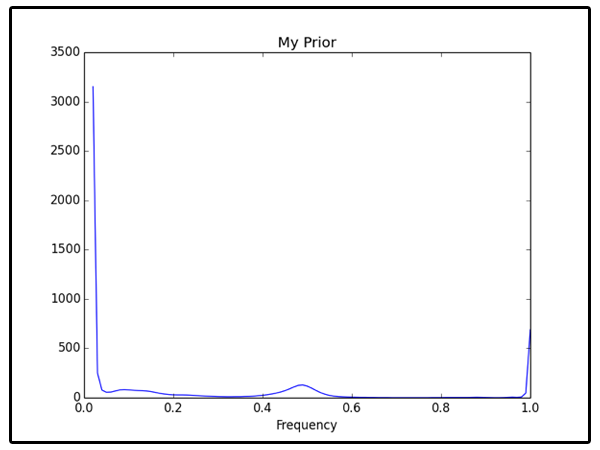
\includegraphics[scale=0.75]{myprior_600.png}
\end{center}

\noindent with a bump at a frequency of 50\% produced by heterozygous variants in the diploid human genome.

\subsubsection{Step 4}

Step 4 wraps the script which computes the SAVI statistics.
In the simple case of comparing sample 2 (tumor) to sample 1 (normal), SAVI adds the following sub-fields to the vcf INFO field:

\begin{itemize}
\tightlist
\item
  \textbf{S1\_P} Savi presence call boolean for sample 1
\item
  \textbf{S1\_PF} Savi posterior for presence or absence for sample 1
\item
  \textbf{S2\_P} Savi presence call boolean for sample 2
\item
  \textbf{S2\_PF} Savi posterior for presence or absence for sample 2
\item
  \textbf{P1\_F} Savi frequency for sample 1
\item
  \textbf{P1\_L} Savi frequency lower bound for sample 1
\item
  \textbf{P1\_U} Savi frequency upper bound for sample 1
\item
  \textbf{P2\_F} Savi frequency for sample 2
\item
  \textbf{P2\_L} Savi frequency lower bound for sample 2
\item
  \textbf{P2\_U} Savi frequency upper bound for sample 2
\item
  \textbf{PD21\_F} Savi frequency delta for sample 2 vs 1
\item
  \textbf{PD21\_L} Savi frequency delta lower bound for sample 2 vs 1
\item
  \textbf{PD21\_U} Savi frequency delta upper bound for sample 2 vs 1
\end{itemize}

\noindent The program does two things. The first is to filter for variants that are present in either sample. The field \texttt{S1\_P}, for instance, is a boolean that gives a presence call for sample 1, while \texttt{S1\_PF} gives the posterior for either the presence or absence.
The default filter in our two sample example looks like this:

\begin{center}
\texttt{( S1\_P = 1 \& S1\_PF < 1e-6 ) | ( S2\_P = 1 \& S2\_PF < 1e-6 )}
\end{center}

\noindent The second thing the program does is to add the rest of the stats without further filtering. Later, in Step 5, we apply an additional filter on \texttt{PD21\_L}, the lower bound of the frequency delta, to find significant variants in one of the reports.\\

\noindent If we had multiple samples, we could make any comparisons we like by adding this information in the \texttt{--compsamp} flag. For example, 

\begin{center}
\texttt{--compsamp 2:1,3:1,3:2}
\end{center}

\noindent would compare 2 to 1, 3 to 1, and 3 to 2.

\subsubsection{Step 5 and Pipeline Output}

Step 5 is a wrapper for SnpEff along with some commands to filter the final reports in various ways.
After annotating genomic features with SnpEff, Step 5 loops over the comma-delimited list of vcf files given in the \texttt{--annvcf} flag, so you can provide as many external annotations as you like.
We typically use a series of vcfs like: 

\begin{Verbatim}
dbSnp138.vcf, \
CosmicVariants_v66_20130725.vcf, \
219normals.cosmic.hitless100.noExactMut.mutless5000.all_samples.vcf, \
cbio.fix.sort.vcf, \
meganormal186TCGA.fix.sort.vcf
\end{Verbatim}

\noindent to annotate variants in dbSnp, Cosmic mutations, and variants in our own ``super normal"---a list of non-significant mutations we've compiled which can appear as significant due to systematic errors. This is an important negative control.\\

\noindent Step 5 also produces reports, in both vcf and tsv format, with various filters:

\begin{itemize}
\tightlist
\item
  \textit{report.all} - the product of the filters heretofore applied
\item
  \textit{report.coding} - filter for variants in the coding region
\item
  \textit{report.coding.somatic} - filter for variants in the coding region;
   discard variants in the meganormals;
   discard common dbSnps;
   discard variants where the normal sample has variant-supporting reads above a certain depth threshhold
\item
  \textit{report.coding.PDfilter} - filter for variants in the coding region;
   filter such that the frequency delta lower bound for tumor vs normal is greater than zero;
   other filters
\end{itemize}

\noindent In practice, you'll probably want to open up Excel and do some of your own filtering on top of the default filters.

\subsection{savi.py Options}\label{savi.py}

\begin{Verbatim}[fontsize=\small]
Usage: savi.py [-h] [--bams BAMS] [--ref REF] [--outputdir OUTPUTDIR]
               [--region REGION] [--names NAMES] [--compsamp COMPSAMP]
               [--steps STEPS] [--ann ANN] [--memory MEMORY]
               [--scripts SCRIPTS] [--mindepth MINDEPTH] [--minad MINAD]
               [--mapqual MAPQUAL] [--maxdepth MAXDEPTH] [--s1adpp S1ADPP]
               [--minallelefreq MINALLELEFREQ] [--annvcf ANNVCF]
               [--buildprior BUILDPRIOR] [--prior PRIOR]
               [--prioriterations PRIORITERATIONS] [--presence PRESENCE]
               [--conf CONF] [--precision PRECISION] [--noindeldepth]
               [--rdplusad] [--index INDEX] [--noncoding] [--noclean]
               [--noerror] [--verbose] [--superverbose]

Arguments:

  -h, --help            show this help message and exit
  --bams BAMS, -b BAMS  comma-delimited list of bam files (by convention list
                        the normal sample first, as in: normal.bam,tumor.bam)
                        (.bai indices should be present)
  --ref REF             reference fasta file with faidx index in the same
                        directory
  --outputdir OUTPUTDIR, -o OUTPUTDIR
                        the output directory (default: cwd)
  --region REGION, -r REGION
                        the genomic region to run SAVI on (default: full
                        range) (example: chr1 or chr1:1-50000000)
  --names NAMES         sample names in a comma-delimited list, in the
                        corresponding order of your bam files (default: names
                        are numerical indicies)
  --compsamp COMPSAMP, -c COMPSAMP
                        comma-delimited list of colon-delimited indices of
                        samples to compare with savi (default: everything
                        compared to sample 1) (example: 2:1 would compare the
                        second bam file to the first) (example: 2:1,3:1,3:2
                        would compare the second to the first, the third to
                        the first, and the third to the second)
  --steps STEPS         steps to run (default: 1,2,4,5 (i.e., all except prior
                        generation))
  --ann ANN             name of the SnpEff genome with which to annotate
                        (default: hg19)
  --memory MEMORY       the memory for the (SnpEff) Java virtual machine in
                        gigabytes (default: 6)
  --scripts SCRIPTS     location of scripts dir (directory where this script
                        resides - use this option only if qsub-ing with the
                        Oracle Grid Engine)
  --mindepth MINDEPTH   the min tot read depth required in at least one sample
                        - positions without this wont appear in pileup file
                        (default: 10). Where the filtering occurs: samtools
                        mpileup post-processing
  --minad MINAD         the min alt depth (AD) in at least one sample to
                        output variant (default: 2). Where the filtering
                        occurs: samtools mpileup post-processing
  --mapqual MAPQUAL     skip alignments with mapQ less than this (default:
                        10). Where the filtering occurs: samtools mpileup
  --maxdepth MAXDEPTH   max per-BAM depth option for samtools mpileup
                        (default: 100000)
  --s1adpp S1ADPP       for filtered report, require the sample 1 (normal) alt
                        depth per position to be less than this (default: 3)
                        (note: this is NOT sample1 alt depth of the given alt
                        but, rather, at the given position). Where the
                        filtering occurs: generating report.coding.somatic
  --minallelefreq MINALLELEFREQ
                        Sgt1MAXFREQ (the allele frequency of any sample not
                        including the first one, assumed to be normal) is
                        greater than this (default: 4) Where the filtering
                        occurs: generating the PD.report file.
  --annvcf ANNVCF       comma-delimited list of vcfs with which to provide
                        additional annotation (default: none). Where it's
                        used: SnpSift
  --buildprior BUILDPRIOR
                        starting input prior when building the prior if step 3
                        is invoked (default: bin/prior_unif01)
  --prior PRIOR         prior to use if step 3 is not run (default:
                        bin/prior_diploid01)
  --prioriterations PRIORITERATIONS
                        the number of iterations for the prior build, if step
                        3 is run (default: 10)
  --presence PRESENCE   the SAVI presence posterior (default: 1e-6). Where
                        it's used: step 4
  --conf CONF           the SAVI conf (default: 1e-5). Where it's used: step 4
  --precision PRECISION
                        the SAVI precision (default: 0). Where it's used: step
                        4
  --noindeldepth        do not include include indel reads in total depth
                        count (SDP) (default: off) (note: asteriks in mpileup
                        are included irrespective of this flag). Where it's
                        used: step 2
  --rdplusad            use reference-agreeing reads plus alternate-calling
                        reads (RD+AD) rather than total depth (SDP) as input
                        to savi (default: off). Where it's used: step 2
  --index INDEX         an index used in naming of output files (default: 0)
  --vcf VCF             (for running step 5 as a stand-alone only) vcf to use
                        as input
  --noncoding           use snpEff to find all transcripts, not just only
                        protein transcripts (default: off). Where it's used:
                        step 5
  --noclean             do not delete temporary intermediate files (default:
                        off)
  --noerror             do not check for errors (default: off)
  --verbose, -v         echo commands (default: off)
  --superverbose        print output of the programs called in each step
                        (default: off)
\end{Verbatim}

\renewcommand\bibname{References}

\begin{thebibliography}{9}

\bibitem{saviref} 
Vladimir Trifonov, Laura Pasqualucci, Enrico Tiacci, Brunangelo Falini and Raul Rabadan.
\textit{SAVI: a statistical algorithm for variant frequency identification}.
\textit{BMC Systems Biology} 2013, 7(Suppl 2):S2 doi:10.1186/1752-0509-7-S2-S2.
 
\end{thebibliography}

\end{document}
